\section*{1.2 One-player game}
\textbf{Let $\mathcal{G} = \langle V, E \rangle$ be a legal graph. A move in a one-player game in $\mathcal{G}$
is a reversal of a single edge, such that the resulting graph is legal.\\
Consider the following problem: given a legal graph $\mathcal{G}$ and an edge $e \in E$, does there exists
a sequence of moves that reverse edge $e$?\\
We proved that if we restrict the above problem to the case where every edge
can be reversed at most once, then the problem is NP-complete (reduction
from 3CNF)\\
Show that the above problem is PSpace-complete.}\\
1. \underline{$\in \textsc{PSpace}$}\\
I will use Savitch's theorem here, more concretely its corollary $\textsc{NPSpace} = \textsc{PSpace}$.\\
Let $G = \langle V, E \rangle$ be the graph on which the only player plays the game and let $e$ be the
winning objective -- the single edge to reverse in order to win the game. There can only be $2^{|E|}$
different stats of the game, so if there exists a sequence of moves reversing edge $e$, there also
exists such sequence not longer than $2^{|E|}$.\\
We can use a totally nondeterministic algorithm, which in each timestep chooses nondeterministically
any edge in the graph such that it can be reversed without invalidating the graph (this can be checked
in polynomial time, even linear $O(|V|+|E|)$ by checking weights inequalities for each node) and reverses it.
This procedure stops after $2^{|E|}$ steps or if no edge can be reversed without invalidating the graph.
If (and only if) any of the nondeterministic runs finds a sequence reversing $e$, then the player has
the winning strategy.\\

\noindent
2. \underline{\textsc{PSpace}-hard}\\
I will show a reduction from QBF in to one-player flow game. I will assume three
things about the formula:
\begin{itemize}
      \item It is in prenex normal form (i.e. all quantifiers preceed the portion
      containing an unquantified Boolean formula). Moreover, let's assume that the
      existental and universal quantifiers alternate -- if it is not the case in the
      original input formula, we can introduce quantifiers with dummy variables, not
      used anywhere in the formula. For instance, $\exists_{x_1} \exists_{x_2}
      \phi(x_1, x_2) \mapsto \exists_{x_1} \forall_{y_1} \exists_{x_2} \phi(x_1, x_2)$
      ($y_1$ is a "dummy" variable).
      \item There are no $\rightarrow$ symbols in the "body" of the formula. Every implication
            can be transformed into an alternative with negation ($a \rightarrow b$ is $\lnot a \lor b$).
      \item All negations in the formula are applied directly to the variables (this
            can be easily ensured with de Morgan's laws).
\end{itemize}
Let
$\forall_{x_1} \exists_{x_2} \forall_{x_3} ... \exists_{x_n}
(y_{1,1} \lor ... \lor y_{1,k_1}) \land (y_{2,1} \lor ... \lor y_{2,k_2}) \land ... (y_{m,1} \lor ... \lor y_{m,k_m})$
be the given quantified boolean formula.\\
I will show a method for constructing the game graph by treating the formula as a composition
of smaller formulas.
The graphs created from any formula will always conform to two invariant assumptions:
\begin{itemize}
      \item All the free variables are provided to the formula as nodes with weight $1$.
            There will also be nodes for negations of the free variables.
            A variable can be set to true by firing its corresponding node.
            It can be set to false by firing its negation's vertex.
      \item A graph for formula $\delta$ contains a node with an outgoing edge of
            weight $1$ which can be reversed (following the games rules) if and only if the
            formula $\delta$ is satisfiable.
            Moreover, this edge will have weight $1$ if $FV(\delta) \neq \emptyset$ and $0$ if
            $FV(\delta) = \emptyset$ ($FV(\delta)$ is the set of free variables in $\delta$).
\end{itemize}
The provided QBF can be decomposed into a tree where every node contains a formula created in a compositional
way from its children.\\
Thus every subformula is of one of the following forms:
\begin{itemize}
      \item $x$ -- a single free variable
      \item $\lnot x$ -- a negation of single free variable
      \item $\theta \lor \delta$, where $\theta$ and $\delta$ are subformulas with no quantifiers, no $\rightarrow$ symbols,
            such that every negation is applied directly to a variable
      \item $\theta \land \delta$, with the assumptions about $\theta$ and $\delta$ as above
      \item $\exists_{x} \psi$, where $\psi$ is a formula, possibly with quantifiers and a potentially non-empty set of
            free variables
      \item $\forall_{x} \psi$, where $\psi$ is a formula, possibly with quantifiers and a potentially non-empty set of
            free variables
\end{itemize}
I will show how to, for each of the above kinds of subformulas, construct a subgraph.\\

\noindent
\underline{$x, \lnot x$}\\
From our assumption that the free variables are provided as nodes with weight $1$,
also the second invariant follows -- the provided node has weight $1$ and is firing
if and only if the variable (or its negation) is set to true.
\begin{figure}[H]
      \centering
      \caption{Node marked $x$ ($\lnot x$) is firing if and only if the provided value for the free variable $x$ is true (false).}
      \begin {tikzpicture}[scale=0.8]
            \node[label=$1$,style={draw=black,circle}] (A) at(0,0) {$x$};
            \path[->] (A) edge node[above] {1} +(-2,0);
      \end{tikzpicture}\\
      \begin {tikzpicture}[scale=0.8]
            \node[label=$1$,style={draw=black,circle}] (A) at(0,0) {$\lnot x$};
            \path[->] (A) edge node[above] {1} +(-2,0);
      \end{tikzpicture}
\end{figure}

\noindent
\underline{$\phi \land \psi$}
\begin{figure}[H]
      \centering
      \caption{
            The node marked \textit{output} is firing if and only if $\phi \land \psi$
            is satisfied with regard to the provided free variables.
            The depicted state of edges corresponds to the initial state of the game.
            Circles with $\phi$ and $\psi$ denote the graphs build for formulas $\phi$ and $\psi$.
            The edges drawn as incoming to $\phi$ or are routed to the nodes corresponding to
            free variables and their negations, the edges coming out from $\phi$ are edges from its
            output node. I will use this convention with all such nested graphs.
      }
      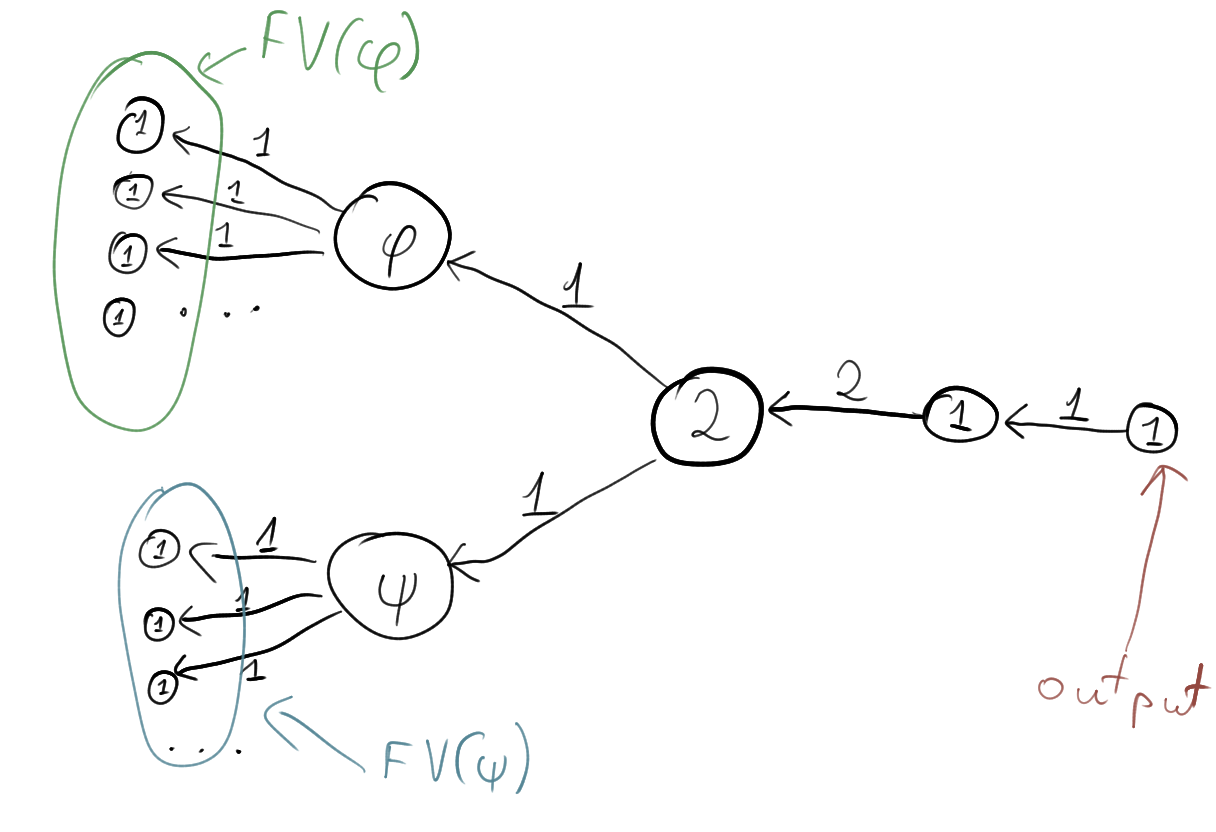
\includegraphics[scale=0.2]{content/graphics/game10.png}
\end{figure}

\noindent
\underline{$\phi \lor \psi$}
\begin{figure}[H]
      \centering
      \caption{
            The node marked \textit{output} is firing if and only if $\phi \lor \psi$
            is satisfied with regard to the provided free variables.
      }
      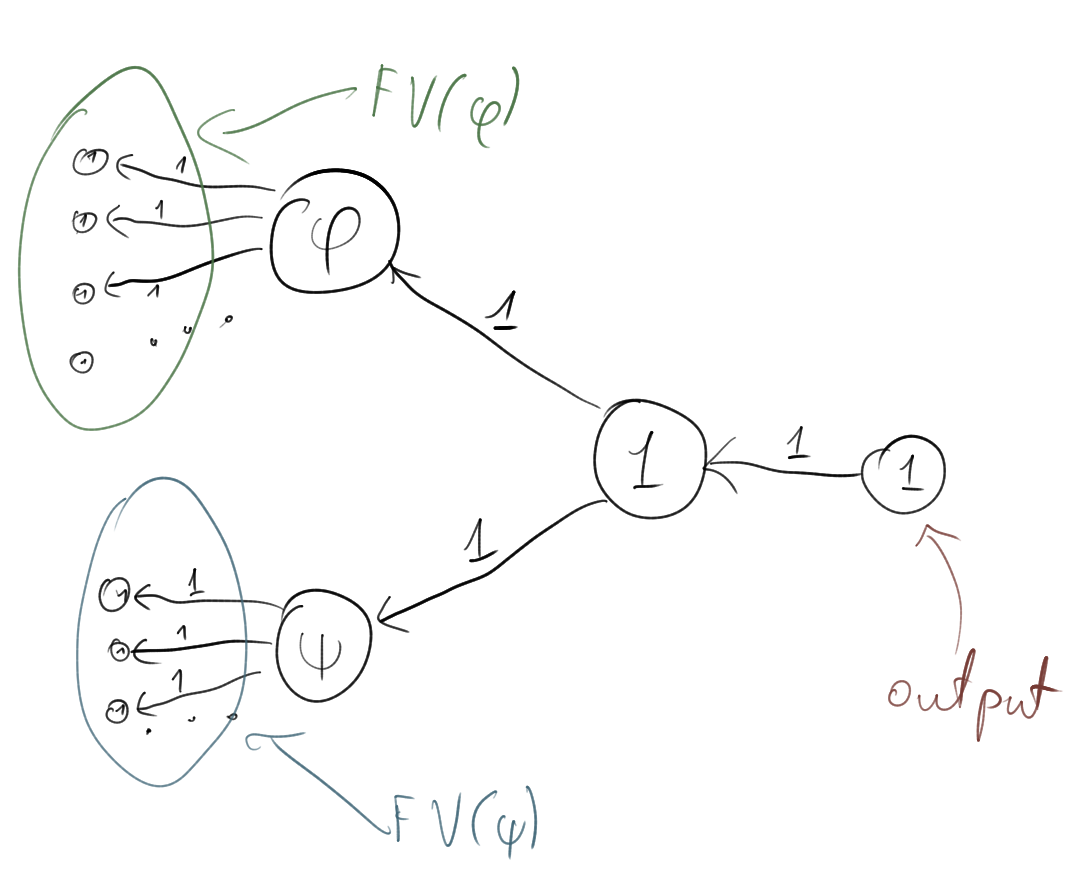
\includegraphics[scale=0.2]{content/graphics/game11.png}
\end{figure}

\noindent
\underline{$\forall_{x} \phi$}
\begin{figure}[H]
      \centering
      \caption{
            This one is more complex. In order to satisfy the entire formula (fire the \textit{output} node),
            the player must separately choose $x$ and $\lnot x$ to be true, satisfy $\phi$ with this choice (i.e.
            fire the output node of $\phi$ nested graph) and fire the corresponding node with weight 3 with a single
            edge of weight 3. Only then can the player propagate the firing towards the \textit{output} node.
            What's important in this construction is that there is only one copy of graph created for $\phi$,
            so the entire graph will not grow exponentially with the number of quantifiers.
            Note that if $FV(\phi) = \{ x \}$ then the \textit{output} node should have weight 0 and its only
            adjacent edge is the edge $e$ that is the objective of the game.
      }
      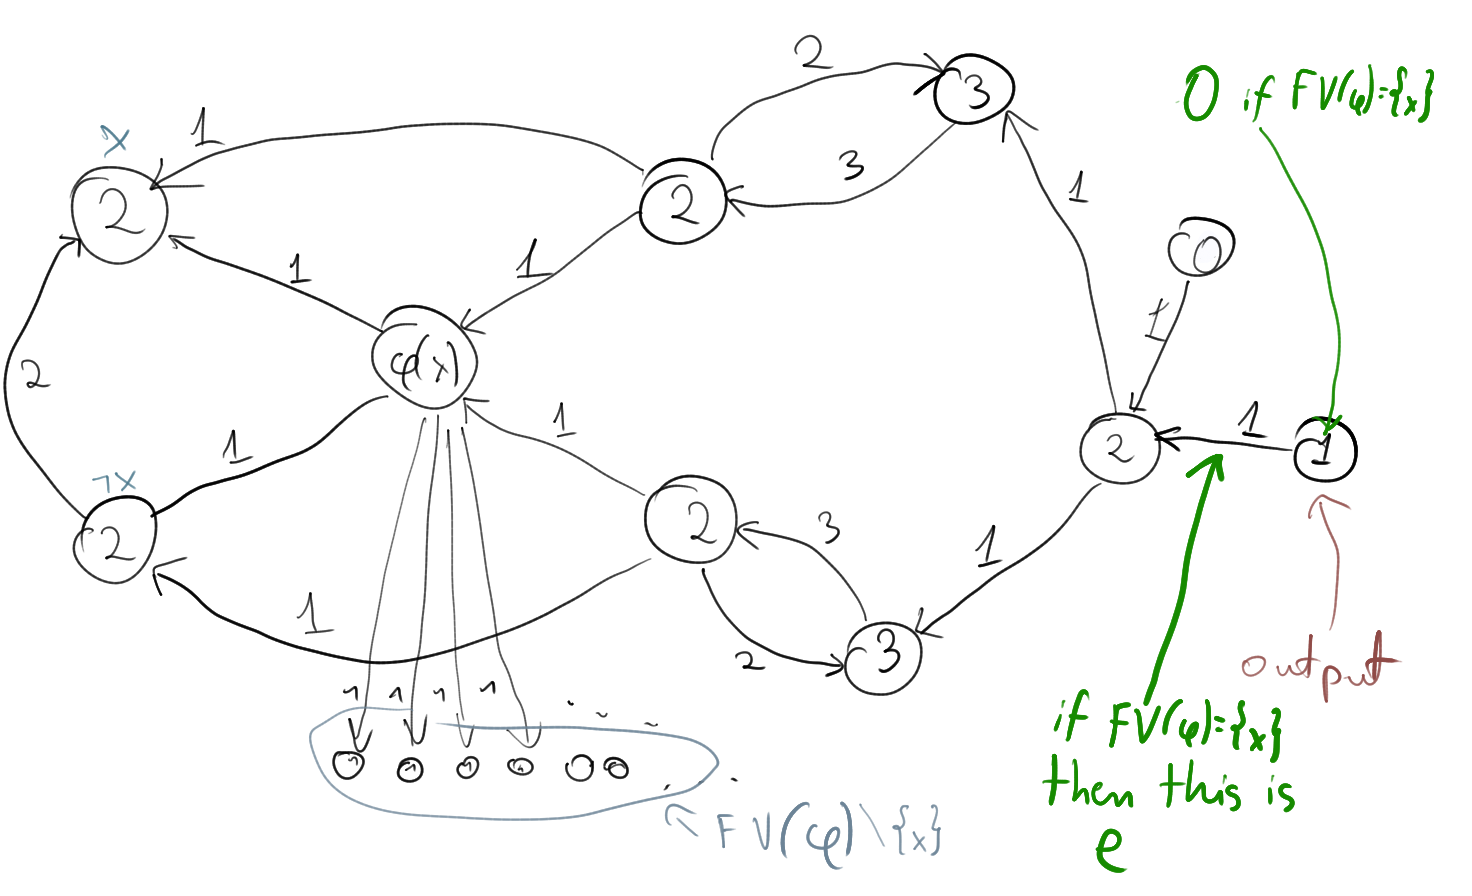
\includegraphics[scale=0.2]{content/graphics/game12.png}
\end{figure}

\noindent
\underline{$\exists_{x} \phi$}
\begin{figure}[H]
      \centering
      \caption{
            The construction is similar as in the previous case ($\forall_{x} \phi$), but to fire the \textit{output}
            node it suffices that the player satisfies $\phi$ with only one choice from $\{x, \lnot x\}$.
      }
      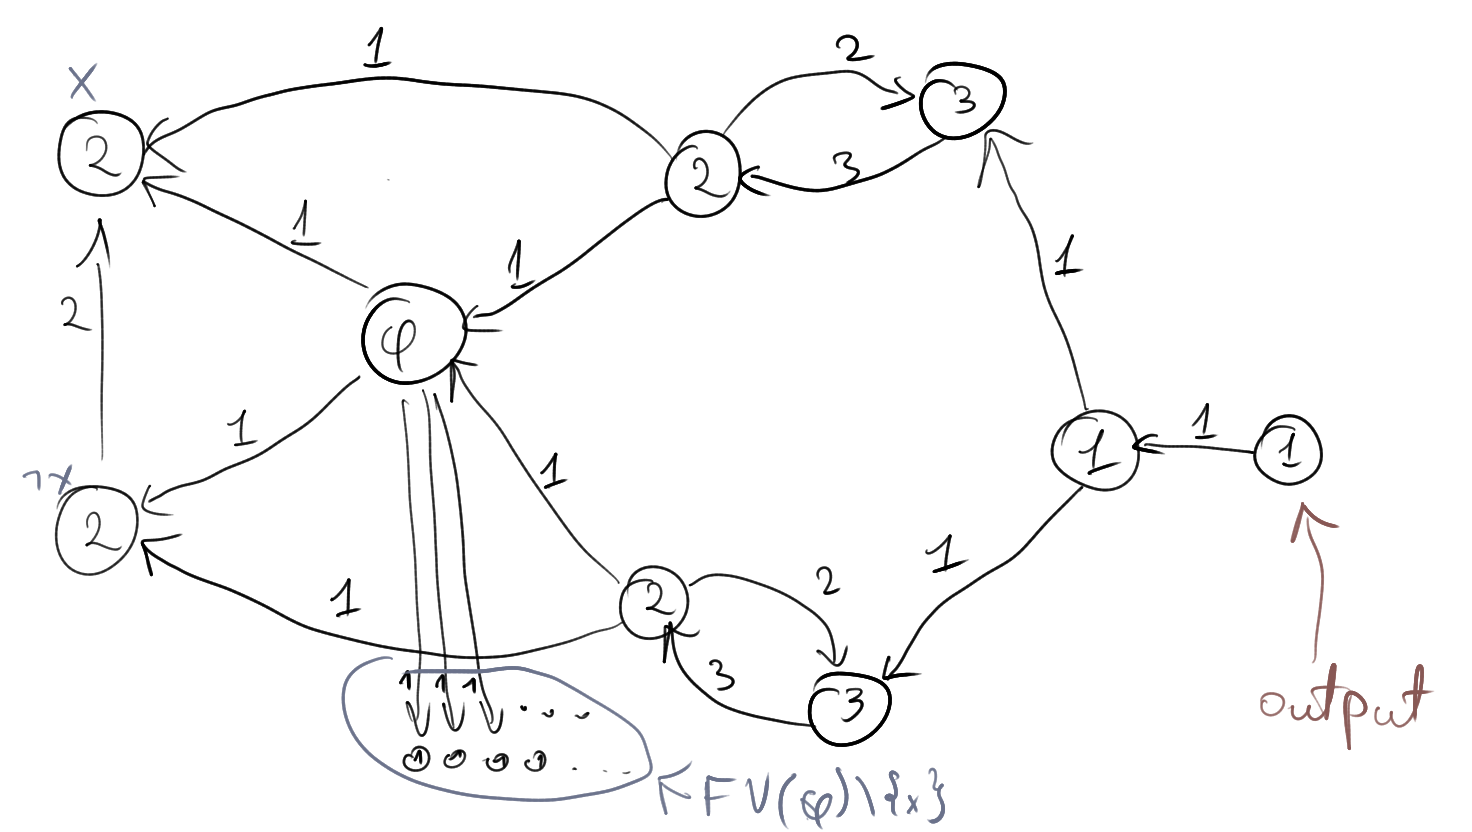
\includegraphics[scale=0.2]{content/graphics/game13.png}
\end{figure}
\begin{figure}[H]
      \centering
      \caption{
            This is an alternative and simpler way to construct the graph for $\exists_{x} \phi$ formula.
      }
      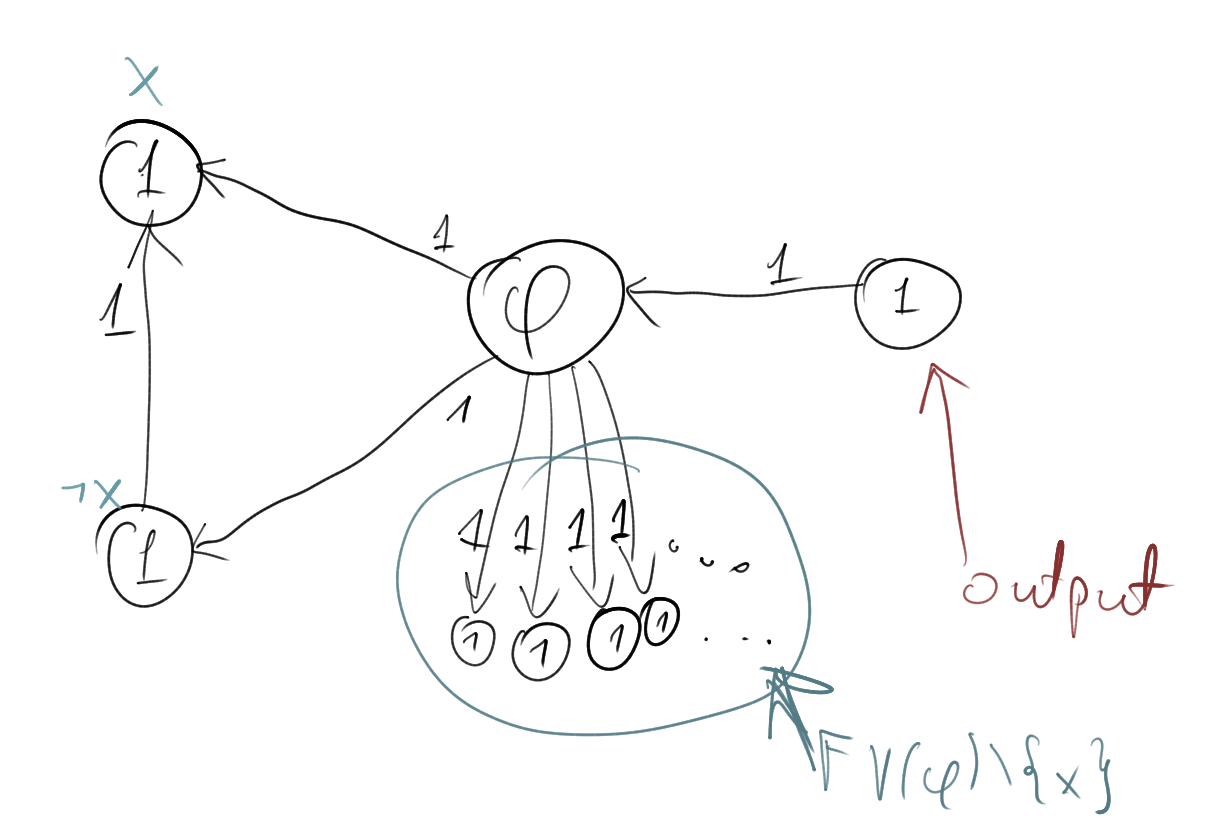
\includegraphics[scale=0.2]{content/graphics/game14.png}
\end{figure}

\noindent
Above I have presented a compositional and recursive way for constructing a graph $G$ and selecting and edge $e$ such that
the only player has a winning strategy in one-player flow game $\langle G, e \rangle$ if and only if the quantified boolean
formula is true.